\documentclass[a4paper,14pt]{extreport}
    \usepackage[left=0.5cm,right=1.5cm,
    top=1.5cm,bottom=1.5cm,bindingoffset=0cm]{geometry}
    
\usepackage{scrextend}

	
	\usepackage{amsmath,amssymb}
	\usepackage{array,tabularx}
	\usepackage{graphicx}
	\graphicspath{{C:/Users/anmnm/Desktop/TeX/images/}}
	\usepackage{moreverb}
	\usepackage{xcolor}
	\usepackage{color}
	\usepackage{hyperref}
	\hypersetup{%
		colorlinks=true,
		linkbordercolor= red,
		urlbordercolor=green,
    }%for hyperrefs
%------------------ 
\usepackage[many]{tcolorbox}
	\newtcbox{\mylib}{enhanced,nobeforeafter,tcbox raise base,boxrule=0.4pt,top=0mm,bottom=0mm,
	  right=0mm,left=4mm,arc=1pt,boxsep=2pt,before upper={\vphantom{dlg}},
	  colframe=green!50!black,coltext=green!25!black,colback=green!10!white,
	  overlay={\begin{tcbclipinterior}\fill[green!75!blue!50!white] (frame.south west)
	    rectangle node[text=white,font=\sffamily\bfseries\tiny,rotate=90] {TYP} ([xshift=4mm]frame.north west);\end{tcbclipinterior}}}

%------------------  
\newcolumntype{Y}{>{\centering\arraybackslash}X}
%------------------  
\usepackage{lstautogobble}  % Fix relative indenting
\usepackage{color}          % Code coloring
\usepackage{zi4}            % Nice font
	\definecolor{bluekeywords}{rgb}{0.13, 0.13, 1}
	\definecolor{greencomments}{rgb}{0, 0.5, 0}
	\definecolor{redstrings}{rgb}{0.9, 0, 0}
	\definecolor{graynumbers}{rgb}{0.5, 0.5, 0.5}

	\usepackage{listings}
	\lstset{
  basicstyle=\ttfamily,
  columns=fullflexible,
  frame=single,
  breaklines=true,
  postbreak=\mbox{\textcolor{red}{$\hookrightarrow$}\space},
  }
%------------------
\usepackage[object=vectorian]{pgfornament} %%  http://altermundus.com/pages/tkz/ornament/index.html
		\usepackage{tikz}
		\newcommand{\sectionlinetwo}[2]{%
		\nointerlineskip \vspace{.5\baselineskip}\hspace{\fill}
		{\color{#1}
		\resizebox{0.5\linewidth}{2ex}
		{{{\begin{tikzpicture}
		\node  (C) at (0,0) {};\node (D) at (9,0) {};
		\path (C) to [ornament=#2] (D);
		\end{tikzpicture}}}}}%
		\hspace{\fill}
		\par\nointerlineskip \vspace{.5\baselineskip}}

  %\newcommand{\img}[4]{\center{\includegraphics[width=#1\linewidth]{#2}}\captionof{figure}{#3}\label{#4}}
\newcommand{\img}[4]{\includegraphics[width=#1\linewidth]{#2}\caption{#3}\label{#4}}


%-----------------------------
\usepackage{tcolorbox}
\tcbuselibrary{skins,breakable}
\usetikzlibrary{shadings,shadows}%preambule
%-----------------------------
\newtcbox{\mybox}[1][red]{on line,
arc=0pt,outer arc=0pt,colback=#1!10!white,colframe=#1!50!black,
boxsep=0pt,left=1pt,right=1pt,top=2pt,bottom=2pt,
boxrule=0pt,bottomrule=1pt,toprule=1pt}

\newtcbox{\xmybox}[1][red]{on line,
arc=7pt,colback=#1!10!white,colframe=#1!50!black,
before upper={\rule[-3pt]{0pt}{10pt}},boxrule=1pt,
boxsep=0pt,left=6pt,right=6pt,top=2pt,bottom=2pt}
%-----------------------------
\usepackage{tikz}
\usetikzlibrary{shapes.callouts}
%-----------------------------
\definecolor{amber}{rgb}{1.0, 0.75, 0.0}
\definecolor{babyblue}{rgb}{0.54, 0.81, 0.94}
%-----------------------------

	\usepackage[framemethod=TikZ]{mdframed}
	\usetikzlibrary{calc}
	\makeatletter
	\newlength{\mylength}
	\xdef\CircleFactor{1.1}
	\setlength\mylength{\dimexpr\f@size pt}
	\newsavebox{\myboxx}
	\newcommand*\circled[2][draw=blue]{\savebox\myboxx{\vbox{\vphantom{WL1/}#1}}\setlength\mylength{\dimexpr\CircleFactor\dimexpr\ht\myboxx+\dp\myboxx\relax\relax}\tikzset{mystyle/.style={circle,#1,minimum height={\mylength}}}
	\tikz[baseline=(char.base)]
	\node[mystyle] (char) {#2};}
	\makeatother
%-----------------------------
\usepackage{verbatim}

\usetikzlibrary{arrows,shapes,backgrounds}
%-----------------------------
\usepackage{multicol}
%-----------------------------
%\usepackage[most]{tcolorbox}
	\definecolor{orang}{RGB}{255,155,0}
	\newtcolorbox[auto counter,number within=section]{caja}[1][]{
	enhanced jigsaw,colback=white,colframe=orang,coltitle=orang,
	fonttitle=\bfseries\sffamily,
	sharp corners,
	detach title,
	leftrule=10mm,
	% What you need %%%%%%%%%%%%
	underlay unbroken and first={\node[below,text=black,anchor=east]
	at ([xshift=-5.5pt]interior.base west) {\Huge  \textbf{!}};},
	%%%%%%%%%%%%%%%%%%%%%%%%
	breakable,pad at break=1mm,
	#1,
	code={\ifdefempty{\tcbtitletext}{}{\tcbset{before upper={\tcbtitle\par\medskip}}}},}
%-----------------------------
%-----------------------------
%-----------------------------
%-----------------------------
%-----------------------------
%-----------------------------
%-----------------------------
%-----------------------------
%-----------------------------
%-----------------------------
%-----------------------------
 




\begin{document}
\begin{center}\xmybox[green]{Мнацаканов Антон} $\quad$ \xmybox[red]{Вар. 5}\end{center}

%####################### 1 #######################
\begin{tcolorbox}[colback=blue!5!white!100,colframe=blue!75!black!90,width=19cm,righttitle=0.5cm, 
title= \center{\Large{\textbf{1}}}]
\begin{center}\bf{Дайте визначення поняття «інтерфейс».}\end{center}
\tcblower
Інтерфейс (англ. interface – засіб спряження, сполучення) це сукупність уніфікованих технічних і програмних засобів, необхідних для підключення зовнішніх пристроїв. Він забезпечує перетворення сигналів МП у сигнали, які сприймаються зовнішніми пристроями, і навпаки, підсилення сигналів та
являє собою апаратні засоби і набір програм передачі даних (уніфікований протокол обміну інформацією).\\

За способом передачі даних інтерфейси можна поділити на синхронні та асинхронні. При синхронному способі передавання даних робота передавального і приймального пристроїв синхронізується спеціальним синхронізуючим сигналом.\\ 

Крім того інтерфейси можна поділити на послідовні та паралельні. У послідовних інтерфейсах передавання (приймання) інформації здійснюється послідовно біт за бітом. При паралельному передаванні даних передається одночасно ціла група бітів. Як правило – це байт або слово.
\end{tcolorbox}


%####################### 2 #######################
\begin{tcolorbox}[colback=orange!5!white!100,colframe=orange!75!black!90,width=19cm,righttitle=0.5cm,
title= \center{\Large{\textbf{2}}}]
\begin{center}\bf{Що представляє собою ARM архітектура?}\end{center}
\tcblower
Архітектура ARM – це RISC архітектура на основі
ліцензованих 32-бітних і 64-бітних мікропроцесорних ядер розробки компанії ARM Limited.
\end{tcolorbox}


%####################### 3 #######################
\begin{tcolorbox}[colback=red!5!white!100,colframe=red!75!black!90,width=19cm,righttitle=0.5cm,
title= \center{\Large{\textbf{3}}}]
\begin{center}\bf{Перелічіть основні недоліки архітектури принстонського типу.}\end{center}
\tcblower
Зростаючі вимоги до продуктивності мікропроцесорних систем спричинили в останні роки перехід до архітектури з гарвардським типом доступу до пам'яті (з двома системними шинами), оскільки кожна пам'ять з'єднується з процесором окремої шиною, що
дозволяє одночасно з читанням або записуванням даних (при виконанні поточної команди) робити вибірку наступної команди. Завдяки такому розподілу потоків команд і даних та поєднанню операцій їх вибірки і виконання реалізується більш висока продуктивність, ніж при використанні архітектури
принстонського типу.
\end{tcolorbox}


%####################### 4 #######################
\begin{tcolorbox}[colback=green!5!white!100,colframe=green!75!black!90,width=19cm,righttitle=0.5cm,
title= \center{\Large{\textbf{4}}}]
\begin{center}\bf{Наведіть класифікацію арифметико-логічних пристроїв за способом дії
над операндами.}\end{center}
\tcblower
Всі виконувані в АЛП операції є логічними операціями (функціями),
які можна поділити на наступні групи:
\begin{itemize}
\item операції двійковій арифметики для чисел з фіксованою крапкою;
\item операції двійкової (або шістнадцяткової) арифметики для чисел з
плаваючою крапкою;
\item операції десяткової арифметики;
\item операції індексної арифметики (при модифікації адрес команд);
\item операції спеціальної арифметики;
\item операції над логічними кодами (логічні операції);
\item операції над алфавітно-цифровими полями.
\end{itemize}
\end{tcolorbox}


%####################### 5 #######################
\begin{tcolorbox}[colback=magenta!5!white!100,colframe=magenta!70!black!90,width=19cm,righttitle=0.5cm,
title= \center{\Large{\textbf{5}}}]
\begin{center}\bf{Опишіть схеми підключення послідовних периферійних інтерфейсів.}\end{center}
\tcblower
\center{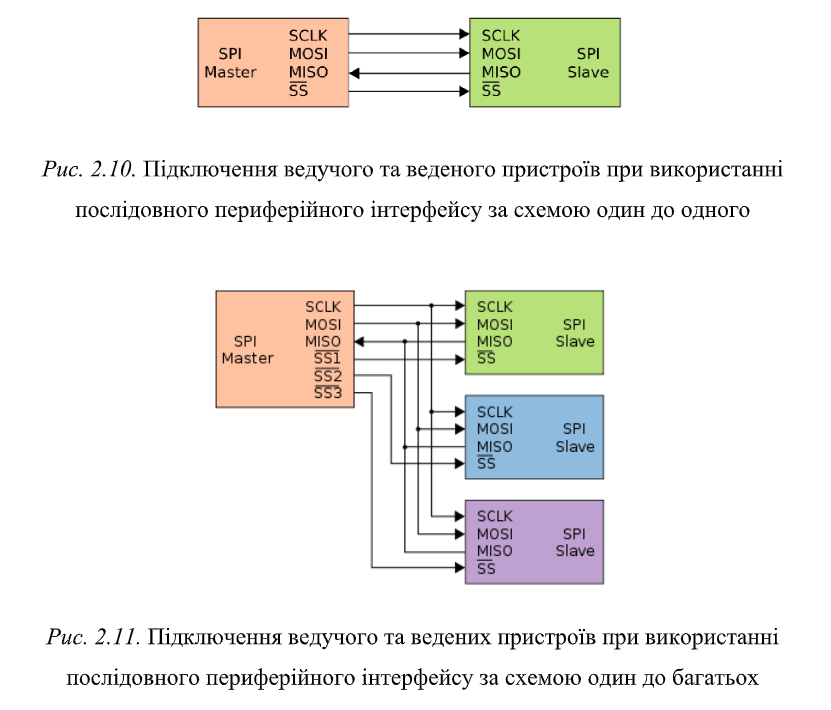
\includegraphics[width=0.7\linewidth]{1.png}}
\end{tcolorbox}



%####################### 6 #######################
\begin{tcolorbox}[colback=gray!5!white!100,colframe=gray!75!black!90,width=19cm,righttitle=0.5cm,
title= \center{\Large{\textbf{6}}}]
\begin{center}\bf{Що являє собою асинхронний послідовний інтерфейс RS-485?}\end{center}
\tcblower
Aсинхронний послідовний iнтерфейс RS-485 може існувати у двох варіантах: двопровідному і чотирипровідному. Двопровідний варіант використовується для напівдуплексної передачі, коли інформація може передаватися в обох напрямках, але в різний час. Для дуплексної передачі використовують чотири лінії зв'язку: за двома інформація передається в одному напрямку, за двома іншими – в зворотному. Недоліком чотирипровідної схеми є необхідність жорсткого визначення ведучого і ведених пристроїв на стадії проектування системи, в
той час як у двопровідній схемі будь-який пристрій може бути як в ролі ведучого, так і веденого. Перевагою чотирипровідної схеми є можливість одночасного передавання і приймання даних, що буває необхідно при реалізації деяких складних протоколів обміну.
\end{tcolorbox}

\end{document}